\documentclass[tikz, border=5pt]{standalone}
\usepackage{pgfplots}
\pgfplotsset{compat=1.17}

\begin{document}
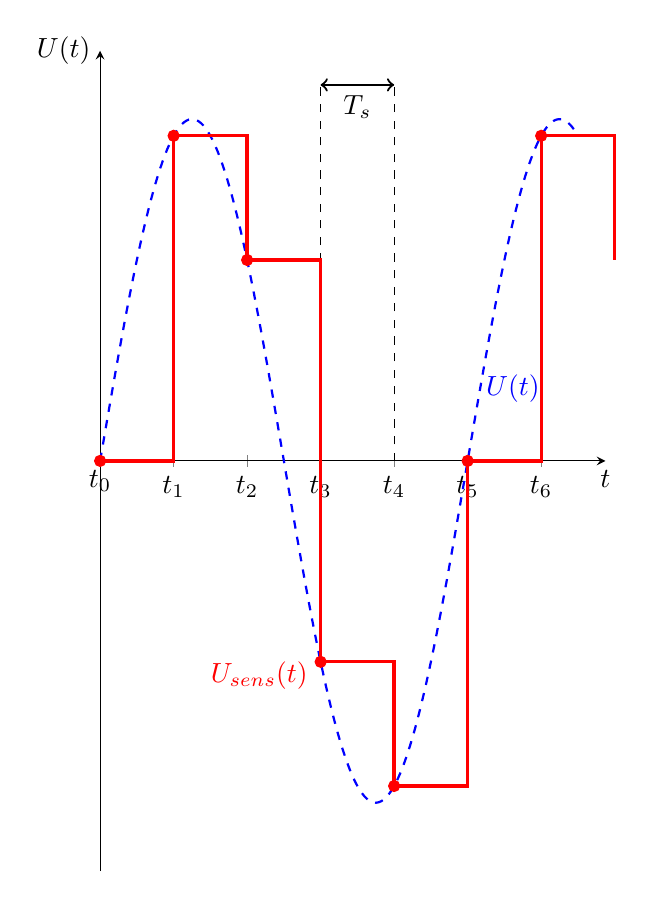
\begin{tikzpicture}
    \begin{axis}[
        width=8cm, height=12cm, % Aspect ratio 2:3
        axis lines=middle,
        xlabel=$t$,
        ylabel=$U(t)$, 
        xlabel style={anchor=north},
        ylabel style={anchor=east},
        xmin=0, xmax=5.5,
        ymin=-1.2, ymax=1.2,
        xtick={0.8, 1.6, 2.4, 3.2, 4.0, 4.8},
        xticklabels={$t_1$, $t_2$, $t_3$, $t_4$, $t_5$, $t_6$},
        ytick=\empty,
        clip=false,
    ]

        % Sampling period Ts
        \draw[dashed] (2.4, 0) -- (2.4, 1.1);
        \draw[dashed] (3.2, 0) -- (3.2, 1.1);
        \draw[<->, thick] (axis cs:2.4, 1.1) -- (axis cs:3.2, 1.1) node[midway, below] {$T_s$};
        
        % Continuous signal (dashed)
        \addplot[blue, dashed, thick, domain=0:5.2, samples=200] {sin(x*90)} node[pos=0.8, anchor=south west] {$U(t)$};

        % ZOH signal
        \addplot[red, very thick, const plot, samples at={0, 0.8, 1.6, 2.4, 3.2, 4.0, 4.8, 5.6}] {sin(x*90)} node[pos=0.45, anchor=north east] {$U_{sens}(t)$};
        
        % Sampling points
        \addplot[red, only marks, mark=*, mark size=2pt, samples at={0, 0.8, 1.6, 2.4, 3.2, 4.0, 4.8}] {sin(x*90)};

        % t_0 label
        \node[below] at (axis cs:0,0) {$t_0$};
    \end{axis}
\end{tikzpicture}
\end{document}
